\documentclass[a4paper]{article}

%% Language and font encodings
\usepackage[english]{babel}
\usepackage[utf8x]{inputenc}
\usepackage[T1]{fontenc}

%% Sets page size and margins
\usepackage[a4paper,top=3cm,bottom=2cm,left=3cm,right=3cm,marginparwidth=1.75cm]{geometry}

%% Useful packages
\usepackage{amsmath}
\usepackage[table,xcdraw]{xcolor}
\usepackage{tabularx,booktabs}
\usepackage{graphicx}
\usepackage[colorinlistoftodos]{todonotes}
\usepackage[colorlinks=true, allcolors=blue]{hyperref}
\usepackage{amsmath}
\usepackage{tikz}
\usepackage{tkz-tab}
\usepackage{caption}
\usepackage{latexsym}
\usepackage{amssymb}
\usepackage{amsmath}
\usepackage{subcaption}
\usepackage{mathtools}
\usepackage{multirow}
\usepackage{listings}
\usepackage{color}
\usepackage{epsfig}
\usepackage{epstopdf}
\usepackage{soul}

%% Useful packages
\usepackage[table,xcdraw]{xcolor}
\usepackage{tabularx,booktabs}
\newcolumntype{C}{>{\centering\arraybackslash}X} % centered version of "X" type
\newcolumntype{b}{X}
\newcolumntype{s}{>{\hsize=.5\hsize}X}
\newcolumntype{v}{>{\hsize=.3\hsize}X}

\definecolor{mygreen}{rgb}{0,0.6,0}
\definecolor{mygray}{rgb}{0.5,0.5,0.5}
\definecolor{mymauve}{rgb}{0.58,0,0.82}


\lstdefinestyle{customc}{
  belowcaptionskip=1\baselineskip,
  breaklines=true,
  frame=L,
  xleftmargin=\parindent,
  language=C,
  showstringspaces=false,
  basicstyle=\footnotesize\ttfamily,
  keywordstyle=\bfseries\color{green!40!black},
  commentstyle=\itshape\color{purple!40!black},
  identifierstyle=\color{blue},
  stringstyle=\color{orange},
}

\lstdefinestyle{customasm}{
  belowcaptionskip=1\baselineskip,
  frame=L,
  xleftmargin=\parindent,
  language=[x86masm]Assembler,
  basicstyle=\footnotesize\ttfamily,
  commentstyle=\itshape\color{purple!40!black},
}

\lstset{escapechar=@,style=customc}

\usetikzlibrary{automata,arrows,positioning,calc}
\usetikzlibrary{shapes,snakes}

% Commands for commenting in inside the text content
\newcommand{\sergio}[1]{\textcolor{brown}{#1}}
\newcommand{\sergiost}[1]{\textcolor{brown}{\st{#1}}}
\newcommand{\franky}[1]{\textcolor{red}{#1}}


%%% TITLE
\title{Komondor: an Event-Based Wireless Network Simulator for Next-Generation IEEE 802.11ax WLANs}
\author{Sergio Barrachina-Mu\~noz and Francesc Wilhelmi}

\begin{document}
\maketitle

\begin{abstract}
Komondor is a wireless network simulator that includes novel mechanisms for next-generation WLANs, such as Dynamic Channel Bonding or enhanced Spatial Reuse. One of Komondor's main purposes is to emulate the behavior of IEEE 802.11ax-2019 networks, which main challenge is spectral efficiency in dense deployments. Furthermore, due to the growing popularity of autonomous systems and the tendency of WLANs to use learning, Komondor is intended to include intelligent agents that make decisions that allow enhancing the network performance. 

In this document we provide an overview of the Komondor simulator, making insight on its main features, its operational mode and its development stages. Komondor has been conceived as an open source tool that contributes to the ongoing research in wireless networks. For that, all the contents are published at the following public repository: \url{https://github.com/wn-upf/Komondor}. Any interested researcher is invited to collaborate.
\end{abstract}

%\tableofcontents

%\listoffigures

%\listoftables

%%%%%%%%%%%%%%%
% INTRODUCTION
%%%%%%%%%%%%%%%
\section{Introduction}
\label{section:introduction}

IEEE 802.11 WLANs are evolving fast to satisfy the new strict requirements in terms of data rate and users capacity. In addition, wireless networks are evolving towards autonomous management, which in many cases is achieved through Artificial Intelligence (AI). Simulating these new characteristics, thus, is crucial to validate their feasibility. For that, we present Komondor \cite{barrachina2017komondor} is an event-based simulator based on COST \cite{chen2002reusing}, a CompC++ library that allows generating discrete event simulations.\footnote{COST main website: \url{http://www.ita.cs.rpi.edu/cost.html}} 
	
Komondor is an open source tool\footnote{Komondor is a long-term and iterative project which goals are mostly focuses in providing a reliable and accurate IEEE 802.11ax simulator. In this document we present its version v1.0, which includes the core functionalities to provide a basic operation.} that is mostly intended to reproduce the novel techniques included in the IEEE 802.11ax-2019 amendment \cite{tgax2017draft}, which is called to become a benchmark in next-generation wireless networks. Furthermore, due to the increasing popularity of learning-based approaches in WLANs, our simulator is being built to allow the inclusion of intelligent agents that make decisions in simulation time. The decision of building a new wireless networks simulator is based on $i)$ the lack of 11ax-oriented simulators that include novel techniques, $ii)$ the need of generating a tool able to simulate intelligent agents behavior and, $iii)$ the difficulty in extending other existing solutions (e.g., ns-3) towards our abovementioned main goals. 	
	
This documents is structured as follows: ...
	
%%%%%%%%%%%%%%%
% SYSTEM MODEL
%%%%%%%%%%%%%%%
\section{Komondor Design Principles}
\label{section:system_model}

\subsection{Architecture}
Komondor aims to realistically capture the operation of wireless networks. Henceforth, it reproduces actual transmissions on a per-packet basis. To that purpose, Komondor is based on the COST library, which allows building interactions between components (e.g., wireless nodes). Such interactions are achieved through synchronous and asynchronous events. While the former are messages explicitly exchanged between components through input/output ports, the later are based on timers. 

In practice, components perform a set of operations until a significant event occurs. For instance, a node that is decreasing its backoff (i.e., current operation) may freeze it when an overlapping node occupies the channel (i.e., an event). Moreover, the node may start a transmission when the backoff timer is over (i.e., a trigger). Figure \ref{fig:cost} shows the schematic of a COST component, which is characterized by its inports and outports, and a set of timers. 
\begin{figure}[h!]
	\centering
	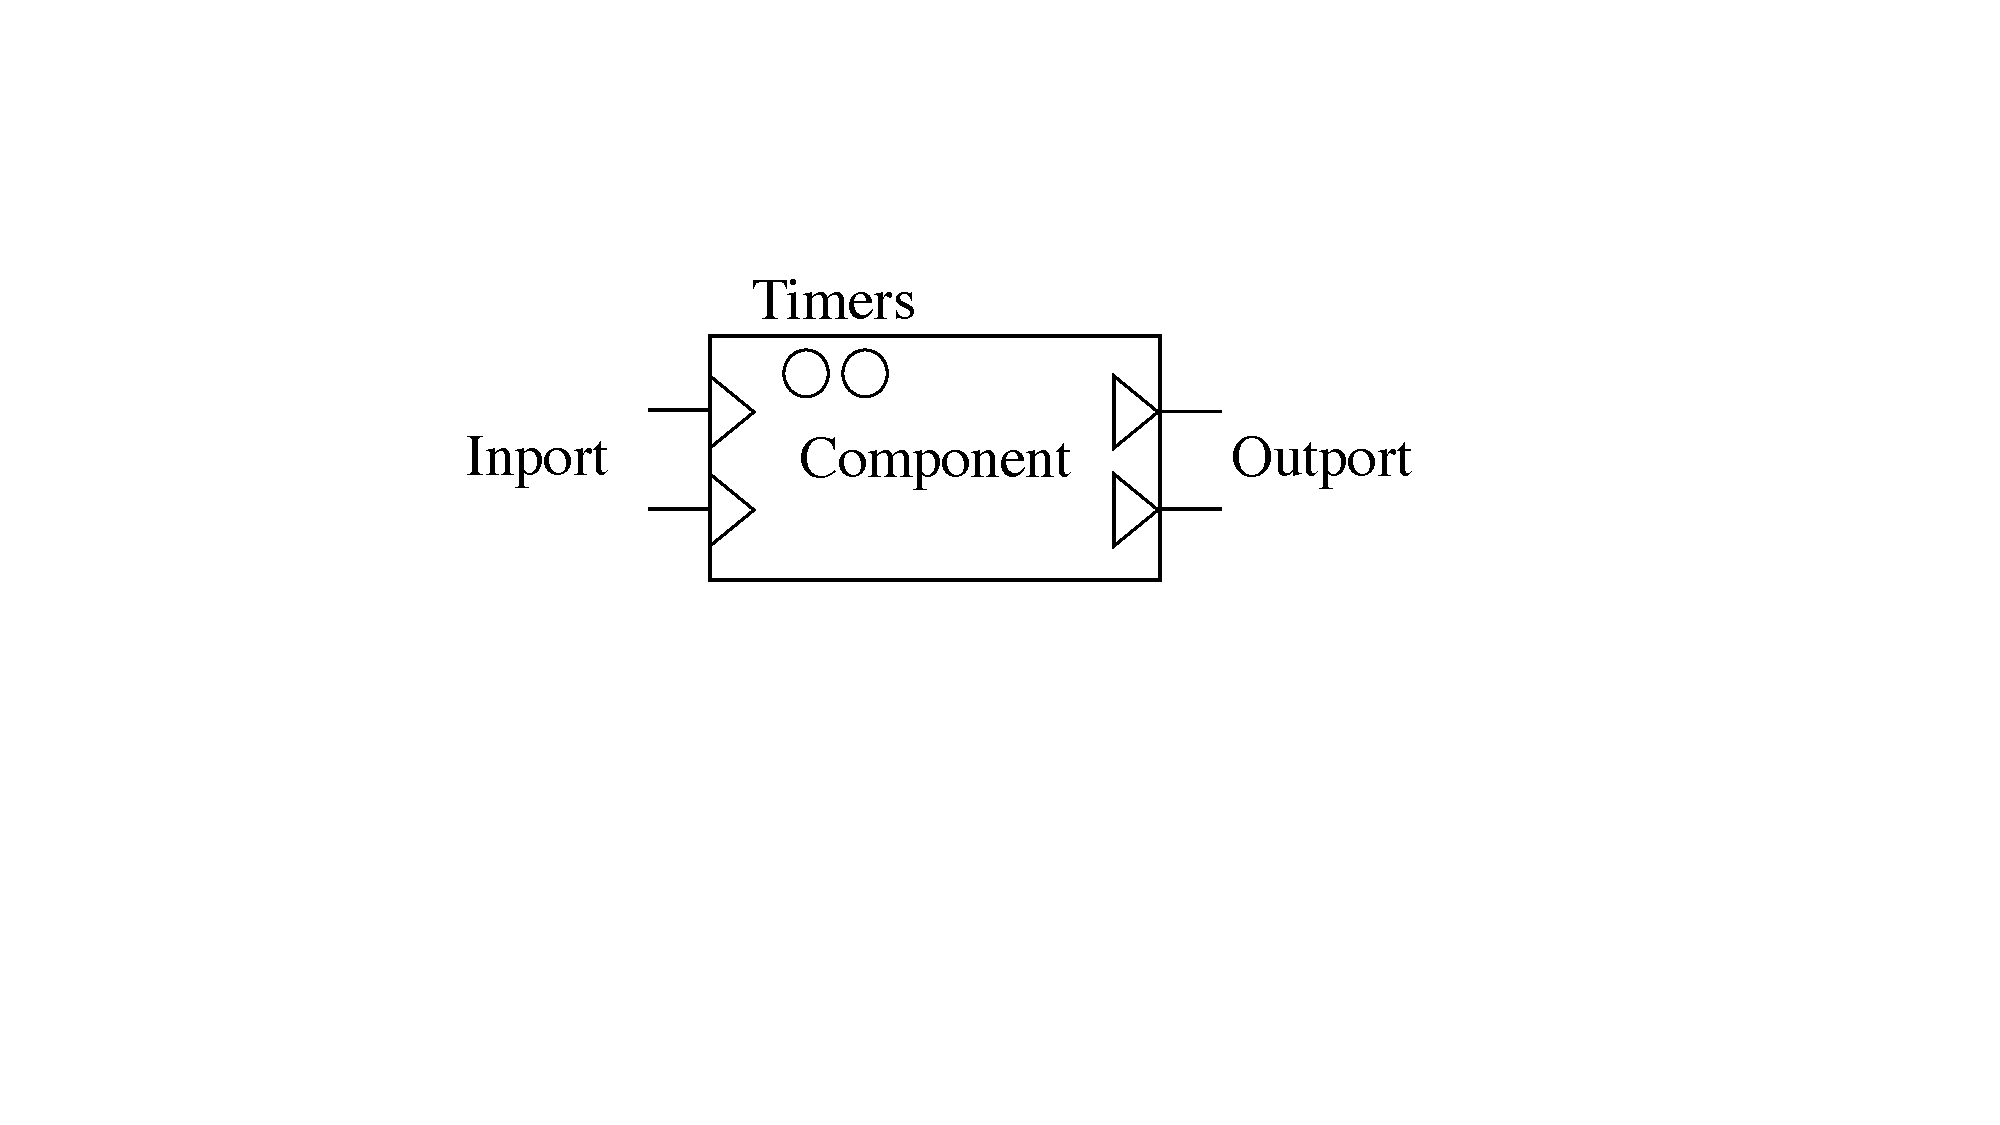
\epsfig{file=images/cost.pdf, width=7cm}
	\caption{COST component. While inports and outports allow to directly communicate with other components, timers trigger events specific to the component.}
	\label{fig:cost}
\end{figure}		

All the abovementioned interactions are simulated based on nodes properties (e.g., location, transmit power, CCA threshold), which allow to frame the wireless operation.

\subsection{IEEE 802.11 Features}
\textcolor{red}{TODO: complete this part.}
The initial version of the Komondor simulator includes the following IEEE 802.11ax features:
\begin{itemize}
	\item \textbf{Distributed Coordination Function (DCF)}: the Carrier Sense Multiple Access with Collision Avoidance (CSMA/CA) captures the basic Wi-Fi operation for accessing the channel. Moreover, Contention Window (CW) adaptation is considered.
	\item \textbf{Channel Bonding (CB)}: several channel ranges can be selected during transmissions in order to maximize the spectrum efficiency.
	\item \textbf{Packet aggregation}: several MPDUs can be aggregated into the same PPDU in order to reduce the generated communication overheads.
	\item\textbf{ Dynamic Modulation Coding Scheme (MCS)}: the MCS is negotiated between any transmitter-receiver pair according to the Signal-to-Interference-and-Noise Ratio (SINR).
	\item \textbf{Ready-to-Send/Clear-to-Send (RTS/CTS) and Network Allocation Vector (NAV)}: nodes exchange packets before transmitting in order to allocate the channel and prevent collisions.
\end{itemize}

Future development stages are considered to include other features such as OFDMA, MU-MIMO transmissions, beamforming, or dynamic transmit power and CST adjustment.

\subsection{Flowchart}
\textcolor{red}{TODO: complete this part and maybe change the title.}
Komondor is composed by several modules that allow performing simulations with a high degree of freedom. Figure \ref{fig:komondor_flowchart} summarizes the operational mode followed by Komondor.
\begin{figure}[h!]
	\centering
	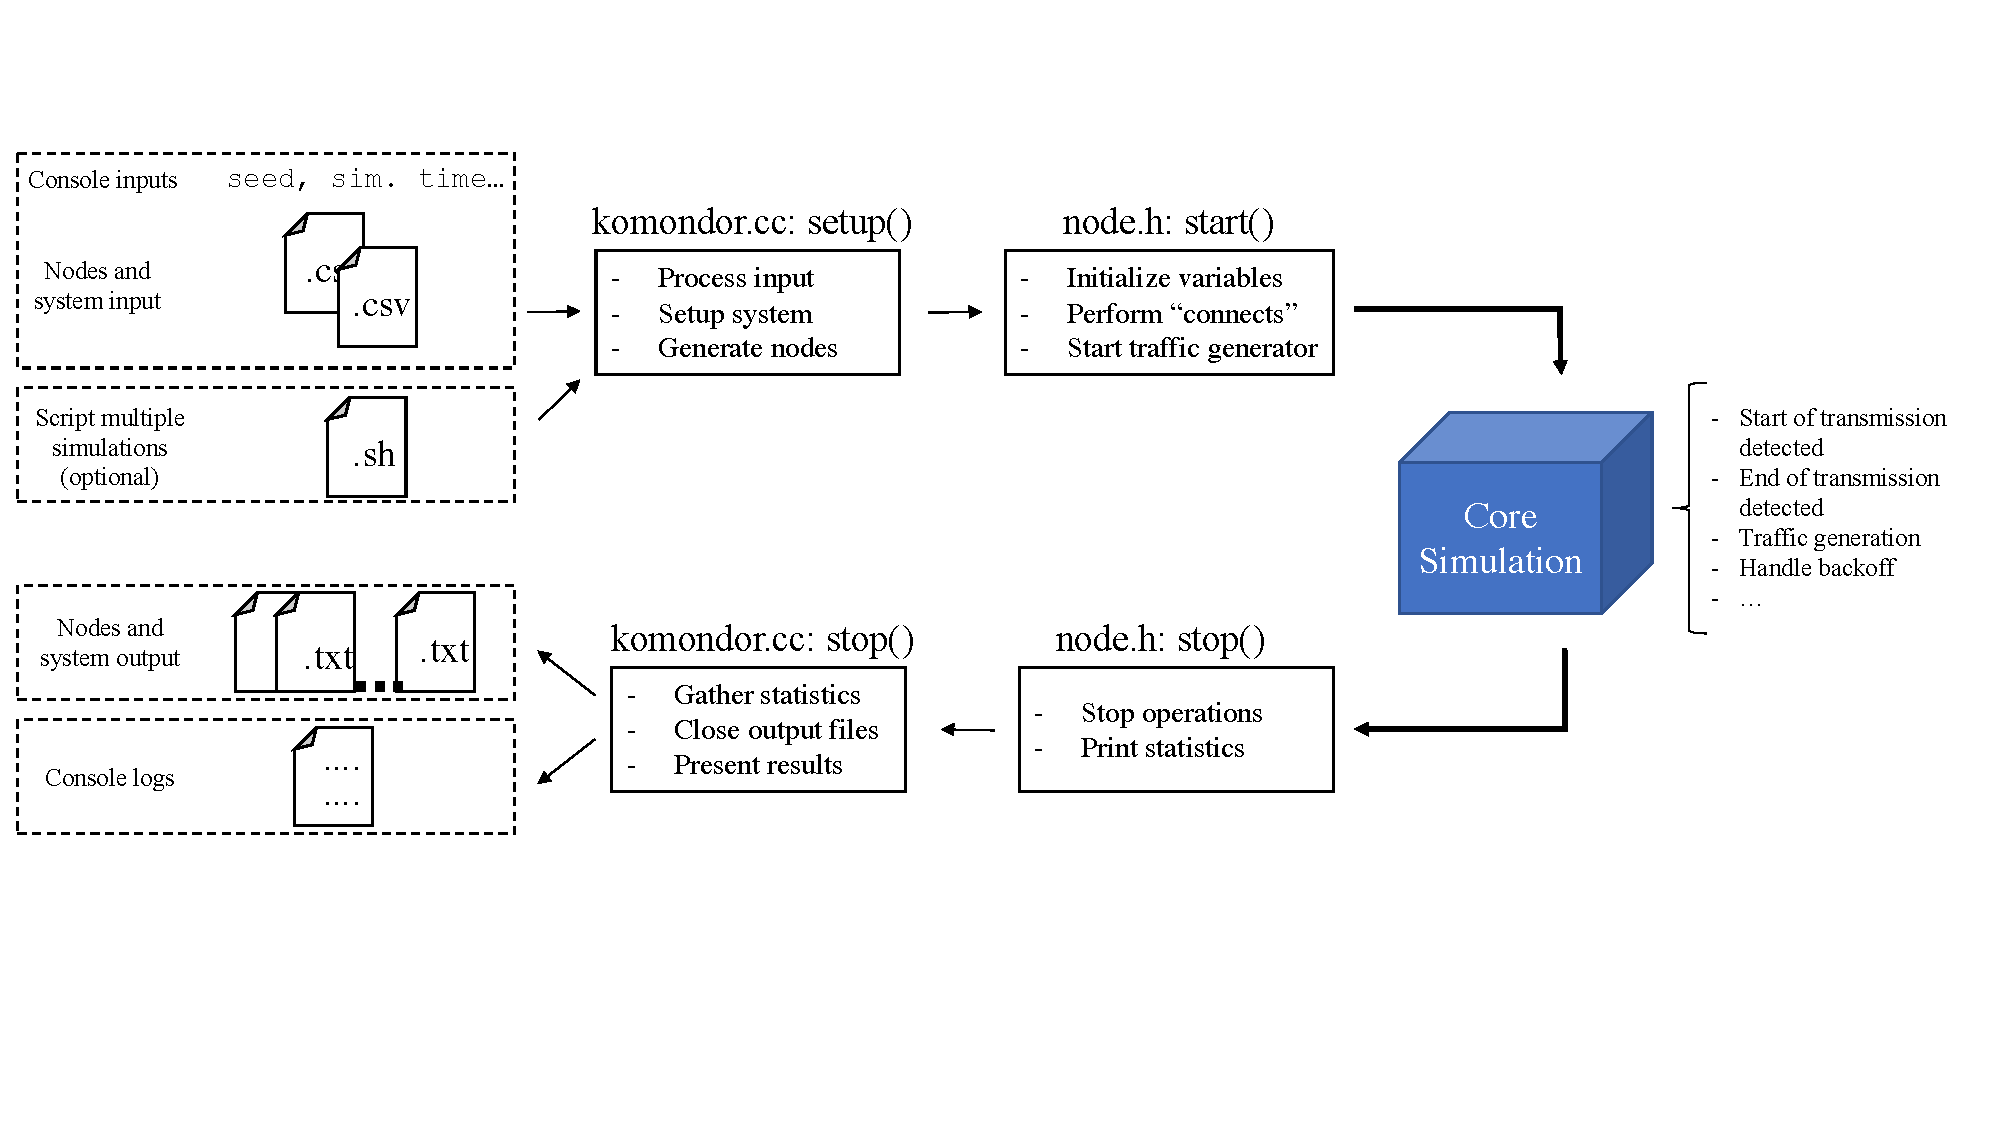
\epsfig{file=images/komondor_flowchart, width=15cm}
	\caption{Komondor flowchart}
	\label{fig:komondor_flowchart}
\end{figure}		

As shown, Komondor receives a set of inputs (nodes information, simulation time, etc.) and initializes the main module, which is in charge of generating the network and gathering useful information regarding the simulation. During the core simulation, nodes interact among each other by sending packets, so that DCF operation is implemented for accessing to the channel. Finally, when the simulation runs out, a set of outputs are generated in order to shed some light on the network performance.

%%%%%%%%%%%%%%%
% VALIDATIONS
%%%%%%%%%%%%%%%
\section{Komondor Main Features Validation}
\label{section:validations}
	In this Section we aim to validate the core operation of Komondor through ns-3 simulations. In addition, a mutual validation is done by considering the Continuous Time Markov Networks (CTMNs) analytical smodel \cite{bellalta2014throughput}. In particular, we use the Spatial-Flexible Continuous Time Markov Network (SFCTMN) \cite{barrachina2018performance}.
	
	With the aim of validating the Komondor operation, we propose a set of key scenarios, illustrated in Figure \ref{fig:scenarios}. The results are summarized in Table \ref{table:results}, which are based on the parameters defined in Table \ref{table:parameters}. 
		 
	\textcolor{red}{TODO:\begin{itemize}
			\item Generate figure containing all the scenarios
			\item Generate table with parameters 
			\item Generate table with results
	\end{itemize}}

%%%%%%%%%%%%%%%
% CONCLUSIONS
%%%%%%%%%%%%%%%
\section{Conclusions}
\label{section:conclusions}
In this document we presented the Komondor simulator, which aims to reproduce the basic operation of IEEE 802.11ax WLANs. Moreover, it has been conceived to allow the utilization of intelligent systems, which is an imperative requirement for next-generation wireless networks. We have validated the basic operation of Komondor through ns-3 simulations and analytical analysis.

This project is expected to move forward for including of novel mechanisms in the 11ax amendment, such as OFDMA, MU-MIMO, and the Spatial Reuse (SR) operation. In addition, intelligent agents are expected to be included for making operations such as Dynamic CB (DCB).

%%% BIBLIOGRAPHY
\bibliographystyle{unsrt}
\bibliography{bib}

\end{document}